\documentclass{article}

\usepackage[final]{neurips_2018}

\usepackage[utf8]{inputenc} % allow utf-8 input
\usepackage[T1]{fontenc}    % use 8-bit T1 fonts
\usepackage{hyperref}       % hyperlinks
\usepackage{url}            % simple URL typesetting
\usepackage{booktabs}       % professional-quality tables
\usepackage{amsfonts}       % blackboard math symbols
\usepackage{nicefrac}       % compact symbols for 1/2, etc.
\usepackage{microtype}      % microtypography

\usepackage{graphicx}
\usepackage{wrapfig}
\usepackage{amsmath}
\usepackage{amssymb}
\usepackage{lipsum}

\newcommand{\Nn}{\mathbf{N}}
\newcommand{\Rr}{\mathbf{R}}
\newcommand{\Pp}{\mathbb{P}}
\newcommand{\Ee}{\mathbb{E}}
\newcommand{\etal}{\textit{et al.}}

\title{Hierarchical reinforcement learning}

\author{%
  Guillaume DALLE \\
  École Nationale des Ponts et Chaussées \\
  \texttt{guillaume.dalle@eleves.enpc.fr} 
  \And
  Clément MANTOUX \\
  École polytechnique \\
  \texttt{clement.mantoux@polytechnique.edu}
}

\begin{document}
% \nipsfinalcopy is no longer used

\maketitle

\begin{abstract}

Hierarchical Reinforcement Learning attempts to solve complex, multiscale problems by breaking them down into smaller subtasks. This decomposition, either provided by an expert or devised automatically, is often necessary to make the learning process faster, or indeed feasible at all. We review different approaches to hierarchical modelling and structure detection in reinforcement learning, with an emphasis on the role of the framework.

\end{abstract}

\section{Introduction}  \label{intro}

\subsection{Problem statement}

Reinforcement learning (RL) deals with problems in which an agent interacts with a (sometimes unknown) environment, and tries to maximize their reward by designing an optimal policy. While standard optimization methods such based on dynamic programming work well in many small-scale situations, learning to perform complex tasks, from robot control to autonomous driving, is still a major challenge.

The reason is that such endeavours are hard to represent using only primitive, atomic actions lasting one time-step. It is better to divide the problem into macroscopic (multi-step) subtasks first, then possibly divide these subtasks into smaller ones, etc.  This multiscale decomposition goes on until reaching the level of primitive actions. Then, the increasingly abstract subtasks can be reconstructed and learned from the bottom up, enabling the agent to solve the initial problem. 
Hierarchical Reinforcement Learning (HRL) aims to integrate this hierarchical decomposition idea into standard RL algorithms. This is meant to speed up the learning process by restricting the search space or giving the learning algorithm more powerful exploration abilities. We will try to give a brief overview of this recent field, with two fundamental questions in mind:
\begin{itemize}
    \item How can one represent and use a given hierarchy of subtasks?
    \item How can one automatically learn the right hierarchical structure for a given problem? 
\end{itemize}

The rest of section \ref{intro} introduces the mathematical framework underlying most RL algorithms. In section \ref{representing}, we present and compare several different ways to express a known hierarchical decomposition. Then, in section \ref{learning}, we tackle the issue of learning an appropriate structure of subtasks, listing both classical and deep learning technniques.

\subsection{(Semi-)Markov Decision Processes and Reinforcement Learning}

Most of the literature on Reinforcement Learning uses the Markov Decision Process (MDP) setting. An MDP is a mathematical model describing the interactions between an agent and an environment. At each discrete time step $t \in \Nn$, the agent finds itself in a state $s_t \in S$, where it can choose an action $a_t \in A$. This action triggers a transition to state $s_{t+1}$ according to conditional probabilities $p(s_{t+1} | s_t, a_t)$, and the agent receives a random reward $r_t$ whose expectation is $r(s_t, a_t)$.

A deterministic policy $\pi: S \to A$ can be evaluated either with the state value function $V^{\pi}: S \to \Rr$, which computes the expected discounted reward when following policy $\pi$ from a given state, or with the state-action value function $Q^{\pi}: S \times A \to \Rr$. The agent's goal is to find an optimal policy, ie. a policy $\pi^*$ reaching the maximum possible value $V^*(s) = \max_{\pi} V^{\pi}(s)$ in each state $s$. Both the value functions and the optimal value functions satisfy Bellman equations similar to:
\begin{equation}
    Q^* (s, a) = r(s, a) + \gamma \sum_{s'}{p(s' | s, a) \max_{a'}{Q(s', a')}}
\end{equation}
Bellman equations form the basis of RL algorithms such as Q-learning \cite{watkins_q-learning_1992}, which allow the agent to learn the transitions and rewards associated with an unknown environment.

Semi-Markov Decision Processes (SMDP) have the same ground rules, except that the actions can last for $\tau > 1$ time steps, leading to duration-dependent transition probabilities $p(s', \tau | s, a)$. They are the adequate tool to represent situations where the agent may perform multi-step combinations of actions in order to achieve a subtask.

\section{Representing the hierarchy} \label{representing}

The basic situation in Hierarchical Reinforcement Learning is the one in which the hierarchy of subtasks is given, most of the time thanks to expert knowledge of the problem at hand. Along the lines of \cite{barto_recent_2003}, we introduce four different proposals to translate the hierarchical structure into a learnable model. We then discuss and compare these approaches.

These proposals will all be illustrated using always the same kind of toy problem inspired by both \cite{dietterich_hierarchical_2000} and \cite{sutton_between_1999}. It consists of a navigation challenge in a room-like grid world (see figure \ref{fig:svi}), where the agent must go from a source cell to a target cell, possibly picking up and dropping off a passenger along the way.

\subsection{Feudal Reinforcement Learning (FRL)}

The first approach we discuss was introduced by Dayan and Hinton \cite{dayan_feudal_1993} and embraces a medieval analogy for absolute hierarchical control. The levels $\ell$ of the hierarchy correspond to partitions $\mathcal{P}_{\ell} = \{R_{\ell, j}, j \in [n_{\ell}]\}$ of the state space into increasingly large regions, each supervised by a manager $m_{\ell, j}$. The bottom level $\ell = 0$ corresponds to the granularity at which the agent can act, and the others correspond to increasing levels of abstraction. At every time step, every active manager $m_{\ell, j}$ (supervising a region containing the agent's state $s$):
\begin{itemize}
    \item receives an order $o_{\ell}^+$ from its super-manager $m_{\ell+1, k}$ (st. $R_{\ell+1, k}  \supset R_{\ell, j}$)
    \item gives an order $o_{\ell}^-$ to its one active sub-manager $m_{\ell-1, i}$ (st. $s \in R_{\ell-1, i} \subset R_{\ell, j}$)
\end{itemize}

In our example, there could be a global manager, then one submanager for each room, and then entry-level managers for each cell. On each level, several orders are available: \texttt{GoNorth}, \texttt{GoSouth}, \texttt{GoEast}, \texttt{GoWest} (orders or actions at level $\ell=0$), and \texttt{FindTarget}, \texttt{GoToRoom($R$)} (abstract orders, available only in the upper levels). The order given by a manager is encoded into the state of its sub-manager, but the sub-manager doesn't understand what the order means at first. Hence the manager also has to set the rewards for his sub-manager, so that it learns which of his actions is best to execute a given order.

The global task by each manager simultaneously applying a Q-learning scheme on its own Q-function $Q[(s, o_{\ell}^+), o_{\ell}^-]$, which it approximates through the rewards decided from above, and which it uses to determine what order will be sent downwards.

\subsection{Hierarchies of Abstract Machines (HAM)}

The second approach we describe is due to Parr and Russel \cite{parr_reinforcement_1998} and draws from the theory of finite automata. Indeed, we add to the MDP a layer of \emph{machines} designed to control it by performing specific subtasks. A machine is defined by a set of states linked by a transition function. There are four machine states: \texttt{Action} (executes an action in the original MDP), \texttt{Call} (calls another machine), \texttt{Choice} (selects a next machine state with given probabilities) and \texttt{Stop} (terminates the execution and goes back to the last call).

\begin{wrapfigure}{r}{5cm}
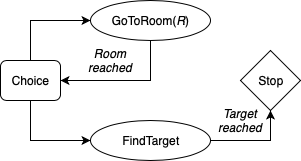
\includegraphics[width=5cm]{images/HAM.png}
\caption{An example of machine in charge of navigation}
\label{fig:HAM}
\end{wrapfigure}

For instance, in our room navigation challenge, there could be a machine (depicted in figure \ref{fig:HAM}) dedicated to navigating towards a given target. It would have two possible calls: either check the current room for the target or go to another one, both being implemented by other sub-machines (which can make use of primitive actions).

If we denote by $H$ the set of machines and by $M$ the original MDP, then the resulting object $H \circ M$ is an SMDP. Its states are pairs of states of $H$ and $M$, and its actions are the possible next states at each machine \texttt{Choice}. After such a decision, the system runs autonomously for several time steps, until another \texttt{Choice} is reached. With a suitable reduction (considering only pairs of states with a \texttt{Choice} component),  $H \circ M$ becomes much less complex than $M$, and can thus be learned quickly with standard MDP algorithms. More details on the learning algorithm (called HAMQ) are given in Parr's PhD dissertation \cite{parr_hierarchical_1998}. 

\subsection{MAXQ decomposition}

\begin{wrapfigure}{l}{7cm}
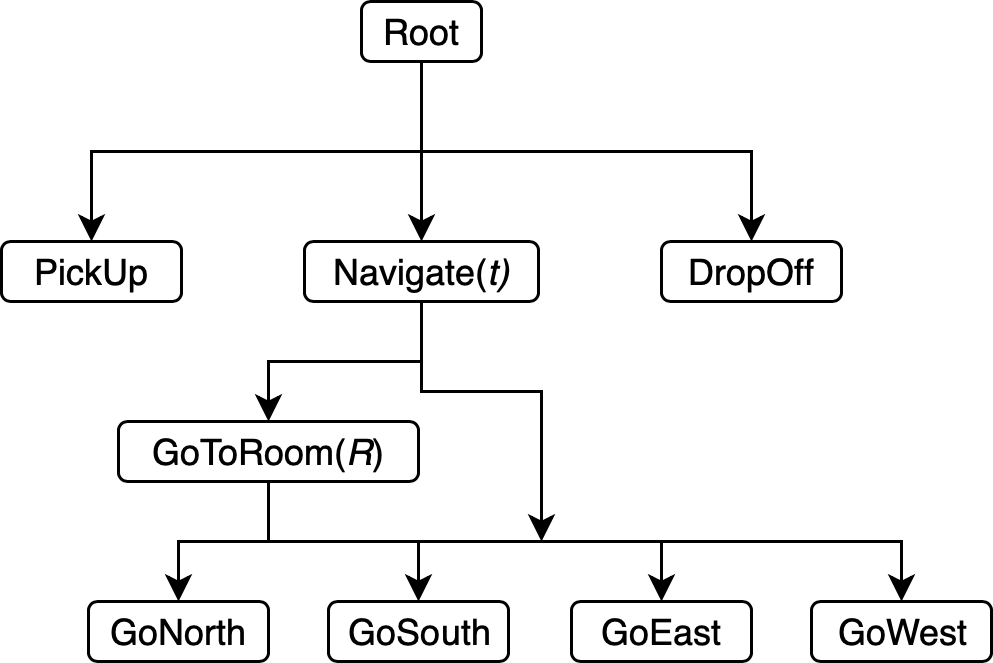
\includegraphics[width=7cm]{images/MAXQ.png}
\caption{Task graph for the MAXQ decomposition}
\label{fig:MAXQ}
\end{wrapfigure}

The third approach we present was imagined by Dietterich \cite{dietterich_hierarchical_2000}, and it is based on a subtask graph. Let us go back to the illustrating example of navigating between rooms, with the added mission of picking up and dropping off an object along the way. Then the subtask graph could look like the one in figure \ref{fig:MAXQ}. The root task is our main challenge, and each child of a node represent a possible subtask this node can use to perform its own mission. The leaves of the graph are primitive actions.

Formally, this is expressed by decomposing the original MDP $M$ into a set of subtasks $M_i$, each being composed of three components: $T_i$ (a termination predicate indicating states where $M_i$ is over), 
$A_i$ (the set of actions or subtasks available to achieve $M_i$) and
$\tilde{R}_i(s)$ (a local pseudo-reward function for terminal states of $M_i$). Given this hierarchical decomposition, a hierarchical policy $\pi$ is a set of policies $\pi_i$ for each subtask, such that $\pi_i$ only uses elements of $A_i$. To apply such a policy, it is necessary to use a stack-based algorithm to keep track of all the subtasks currently executing.

Let us define the projected value function $V^{\pi}(s, a)$ as the expected cumulative reward of executing $\pi_a$ from state $s$ until subtask $M_a$ is over. A key observation is that each subtask $M_i$ where the hierarchical policy $\pi$ is applied defines a SMDP. In this SMDP, the expected reward $r(s, a)$ of each action $a \in A_i$ is equal to its projected value function $V^{\pi}(a, s)$. Furthermore, the Bellman equations here are decomposition equations:
\begin{equation}
    Q^{\pi}(i, s, a) = V^{\pi}(s, a) + C^{\pi}(i, s, a) \quad \text{and} \quad V^{\pi}(s, i) = \begin{cases} Q^{\pi}(i, s, \pi_i(s)) & \text{composite $i$} \\ r(s, i) & \text{primitive $i$} \end{cases}
\end{equation}

In other words, the reward induced by policy $\pi$ on subtask $i$, if it starts on state $s$ with action $a$, can be decomposed into the projected value of state $s$ in subtask $a$ plus a certain completion function.
Therefore, all that is needed to reconstruct the value function are the quantities $[V^{\pi}(a, s)]_s$ for all primitive actions $a$ and $[C^{\pi}(i, s, a)]_{s, a}$ for all composite subtasks $i$. This is at the heart of the recursive MAXQ-0 algorithm, which learns a recursively optimal policy by iteratively updating the $V^{\pi}$ and $C^{\pi}$ values in a stochastic approximation scheme. The MAXQ-Q extension deals with the general case of non-zero pseudo-rewards $\tilde{R}$, which can speed up learning by directing the search.

\subsection{Options}

The fourth approach we detail is the options framework, which was introduced by Sutton, Precup and Singh \cite{sutton_between_1999} and is the basis of much of the modern research on HRL. It forms an extension of the classical MDP setting, where we consider sequences of actions with extended time durations, the so-called \textit{options}.

\begin{wrapfigure}{r}{3.5cm}
    \centering
    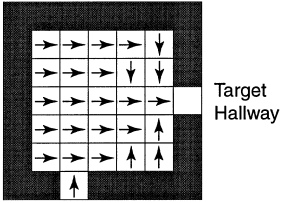
\includegraphics[width=3.5cm]{images/single_option.png}
    \caption{Policy for a single option in the four-room problem. \small \it Image from \cite{sutton_between_1999}.}
    \label{fig:single-option}
\end{wrapfigure}

Formally, we define an option $\omega \in \Omega$ as a tripel $(\mathcal{I}_\omega, \pi_\omega, \beta_\omega)$. The initiation set $\mathcal{I}_\omega \subset \mathcal{S}$ is the set of states where the option is available. Once an option is selected, the agent follows the non-deterministic policy $\pi_\omega$, until the option stochastically terminates with probability $\beta_\omega$ depending on the current state. Primitive actions are then special cases of options that always terminate after one step. Note that the policies $\pi_\omega$ can  depend on the history of states, actions and rewards since the initiation of the option (and not only on the current state $s_t$), which makes it "semi-Markov". The authors in \cite{sutton_between_1999} illustrate the notion of option with the example of the four-room navigation problem. We reproduce in figure \ref{fig:single-option} the subpolicy of an option for moving from one (abstract) room to another.

With these notations, an episode unfolds as follows: the agent picks an option to start with, and follows its policy until it terminates, then it chooses another option, and so on until termination. The options are chosen with a \textit{policy over options} $\pi_\Omega : \mathcal{S} \times \Omega \rightarrow [0, 1]$. An MDP endowed with an options set $\Omega$ and a policy $\pi_\Omega$ is thus an SMDP : the actions of the SMDP are the options in the MDP.
The value functions easily generalize: for instance we can define the option-value function $Q^{\pi_\Omega} : \mathcal{S} \times \Omega \rightarrow \Rr$ and the optimal option-value function $Q^*_\Omega$ as follows :
\begin{equation}
\begin{cases}
Q^{\pi_\Omega}(s, \omega) = \Ee[r_1 + \gamma r_2 + \gamma^2 r_3 +  ... \mid s_0 = s, \omega_0 = \omega] \\
Q^*_\Omega(s, \omega) = \max_{\pi_\Omega} Q^{\pi_\Omega}(s, \omega)
\end{cases}
\end{equation}

\begin{wrapfigure}{r}{7cm}
    \centering
    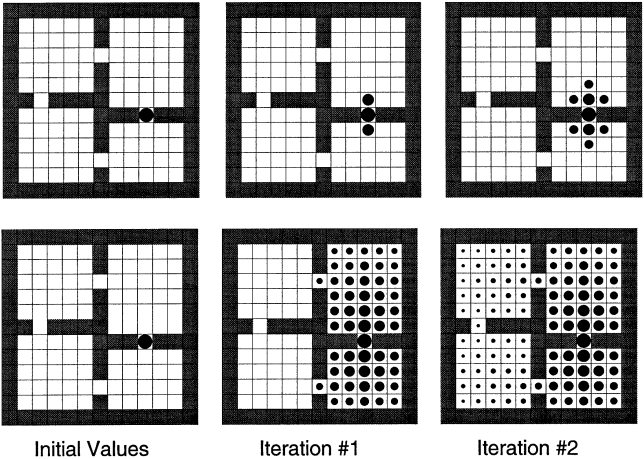
\includegraphics[width=7cm]{images/SVI_options.png}
    \caption{Synchronized Value Iteration with options. \small \it The grids display the value of each state at each iteration. The first row shows the classical MDP value iteration, and the second row shows the same result with hallway-reaching options. The value propagates much faster in the second setting.}
    \label{fig:svi}
\end{wrapfigure}

These values are suboptimal compared with the MDP's classical value functions since the primitive actions may not be available as options : this is the price of the abstraction. Yet, these functions satisfy generalized Bellman equations which can be used to derive learning algorithms.

In the original article \cite{sutton_between_1999}, the options structure is assumed to be known. In this situation, the authors show that well selected options drastically speed up the convergence of estimation algorithms. In figure \ref{fig:svi}, we show their experiment in the four rooms problem. The Synchronized Value Iteration converges much faster in the MDP with options than in the classical setting.

\subsection{Comparison of the frameworks}

We now discuss the merits and drawbacks of the four frameworks introduced above, by comparing them along several axes. This comparison is performed essentially with respect to the original articles introducing the frameworks, regardless of later developments.

\paragraph{Information to supply} The differences between the input requirements of these methods are essential, because structure definition is the part often requiring problem-specific knowledge. In this regard, the options framework is more demanding than the others, because specifying an option means defining an entire local policy. Meanwhile, in the HAM or MAXQ formulation, all that is needed is a description of the subtasks and their mutual dependencies: the means to achieve them are then learned automatically. On the other hand, expliciting the graph structure of subtasks can be quite challenging. This is especially true for FRL, where the link between descending orders and manager-decided rewards is never made concrete.

\paragraph{Convergence} While the FRL article remains vague about convergence issues, the papers introducing HAM, MAXQ and the options each give a justification of convergence for their respective learning algorithm. However, these strongly differ in the properties of the limit policy. While SMDP learning algorithms for HAM and options converge to a hierarchically optimal policy (that is, the best possible policy within the limits of the given hierarchical structure), MAXQ-Q only converges to a recursively optimal policy (that is, a hierarchical policy such that for each task $M_i$, $\pi_i$ is locally optimal given the policies $\pi_a$ chosen for its subtasks $a$). This enables subproblems to be solved regardless of the context, at the price of a possible loss in efficiency.

\paragraph{Mathematical complexity} In philosophical terms, as \cite{jong_utility_2008} points out, there is a great divide between the options framework and the three others we presented. As long as they are made available in addition to primitive actions, options only widen the horizon of RL algorithms, hoping to perform more targeted exploration and thus hasten convergence: the added complexity brings acceleration. Conversely, FRL, HAM and MAXQ are designed to heavily constrain the search space, thus reducing the number of possibilities to check in each iteration of the learning algorithms: here the acceleration is due to simplification. To go even further, \cite{dietterich_hierarchical_2000} formally describes a series of 5 conditions allowing state abstraction within the MAXQ temporal abstraction framework, which works towards even more simplification thanks to a systematic reduction method.

\paragraph{Implementation complexity} Even though on the theoretical level, options increase the complexity of the action space, on the practical level they seem much easier to implement, because they require no recursive structure. Since the options considered are generally semi-Markov (depending on a whole chunk of history), defining an option over options just means defining a more complex option, which is still semi-Markov. This may partly justify the success of options compared with FRL, HAM and MAXQ: with them, there is no need to program a complex structure of managers / machines / subtasks or the intricacies of the MAXQ-Q learning algorithm.

Other ideas: interruptions

\section{Learning the hierarchy} \label{learning}

Now that we have surveyed several methods to represent a given hierarchy of subtasks, we have to ask how to learn one automatically. We will present a few approaches in detail, spread across multiple frameworks and covering both classical and deep learning techniques.

\subsection{Classical approaches}

We first present various proposals from the 2000's that make no use of neural networks. They are grouped by choice of modeling framework.

\subsubsection{Bottleneck and subgoal states for option discovery}

Sutton \etal's options formulation \cite{sutton_between_1999} is by far the most widely used when trying to learn the hierarchical structure of a task, because it lends itself naturally to the definition of subgoals. Subgoal states are interesting milestones on the way to the endgoal, for instance because they are \textit{bottlenecks} between two parts of the state space. We present several heuristics aimed at automatically discovering such states, on the basis of a collected history of trajectories.

The first type of methods uses intuitive threshold criteria to distinguish the most promising states. In order to select emergent features defining temporally extended behaviours, \cite{digney_learning_1998} proposes two metrics: high reinforcement gradient (ie. immediate reward) and high frequency of visits. Multiple-instance learning is used by \cite{mcgovern_automatic_2001} to detect subgoals: successful trajectories are considered as bags containing at least one positive sample, while failed trajectories contain only negative sample. The relative novelty concept of \cite{simsek_using_2004} suggests that bottleneck states are recognizable because the states that follow them in the trajectories are often more frequently visited in the last time steps than the states preceding them.

Another category of approaches makes use of the graph structure induced by collected trajectories on the state space, which is an approximation of the underlying MDP transition scheme. One possibility is to look for interesting minimum cuts in this graph (\cite{goos_q-cutdynamic_2002}, \cite{simsek_identifying_2005}), which can be thought of as shallow frontiers between large areas, crossed by a sizeable flow of trajectories. Another way is to cluster the graph, as is done in \cite{mannor_dynamic_2004}, looking for clusters that are comparable in size, weakly connected with one another and have states with similar values: paths between elements of these clusters are then learned as options.

Note that when working with options, simply finding a subgoal is not enough: the local policy allowing to reach it must also be computed. In the articles listed above, this is often done separately, e.g. with the \textit{experience-replay} method of \cite{lin_self-improving_1992}. This was introduced as an improvement to standard algorithms such as Q-learning, enabling them to better exploit past experiences by reusing them in the stochastic approximation if they are in line with the current policy. In particular, experience replay makes it possible to learn options simply by looking back on previous trajectories.

\subsubsection{Subgoal discovery for feudal structures}

Here we present a procedure for learning options that we think is closely related to a feudal view of HRL: the HASSLE algorithm of \cite{bakker_hierarchical_2004}. It is described for a two-layer hierarchy consisting of one high-level policy $\pi^H$ (a manager) and several low-level policies $\pi_i^L$ (or sub-managers, or options). The high-level policy only sees the current \textit{abstract observation} $o_s^H$, choosing at each time step the abstract observation $o_g^H$ it wants to see next. This couple $(o_s^H, o_g^H)$ is then passed along to the lower-level policies, which are in charge of reaching this desired abstract observation. Each $\pi_i^L$ stores a capability value $C_i(o_s^H, o_g^H)$, which quantifies its potential to reaching subgoal $o_g^H$ from $o_s^H$, and makes it more or less likely to be selected. Crucially, when $\pi_i^L$ is indeed selected, this capacity value is increased or decreased by the higher-level policy depending on whether or not $\pi_i^L$ has achieved the subgoal: this is the equivalent of managers rewarding their subordinates for executing the orders. Both high-level and low-level policies are learned simultaneously using standard routines such as Q-learning.

\subsubsection{Hierarchy building in in factored MDPs}

While the previous methods were applicable to general MDPs, having more hypotheses on the structure of the problem can help design more relevant algorithms. Here we list a few approaches developed in the framework of factored MDPs, where the state variable is represented by a vector $(s^1, ..., s^k)$.

The HEXQ algorithm of \cite{hengst_discovering_2002} defines an order among the coordinates of the state, which depends on each coordinate's frequency of change: in particular, the factor variable that changes most often (ie. the position of the agent, as opposed to the location of the passenger or the destination) will be associated with the lowest level of the hierarchy. Its possible values are then grouped into connected components, or regions, which will contribute to define abstract states for the next hierarchical level. These regions only model a part of the state information, therefore they also possess so-called exits, ie. actions that lead to changes in higher-level factor variables. The abstract actions available at the upper level are the policies leading to region exits at the lower level. Thus, the HEXQ decomposition algorithm can be easily expressed with the MAXQ formalism, and it exploits the connection between temporal abstraction and state abstraction that was suggested in \cite{dietterich_hierarchical_2000}.

\cite{jonsson_causal_2006} goes a bit deeper in the modeling of factor variable dependencies. The use of Dynamic Bayesian Network, a type of probabilistic graphical model, enables the authors to express non-linear structures of influence between variables (as opposed to HEXQ which merely orders them). Using this information, they learn options aimed at reaching each exit context by expressing them as the solution to a sub-MDP with reduced (and abstracted) state and action spaces.

\subsubsection{Intrinsic motivation}

The method detailed in this section was formalized by \cite{chentanez_intrinsically_2005}. It doesn't assume that the exploration of the environment is driven by any specific problem, but rather that its purpose is to learn and store generic skills. Those skills may then be reused in solving a wide variety of challenges.

To perform intrinsically motivated RL, the agent maintains a hierarchy of learned skills, which will grow over time. During exploration, as soon as a \textit{salient state} is encountered (a situation which we suppose can be instantly recognized), the agent will define an option to reach it. Therefore, at first, only the subgoal of the option is known, but a system of intrinsic rewards will allow the agent to learn the paths leading to this subgoal (thus extending the initiation state and option policy) as the exploration continues.

As a final remark, note that contrary to the other option-related methods we presented, this algorithm can and should be executed online. Indeed, the mixture of external and intrinsic rewards strike a balance between solving the global problem and refining local options.

\subsubsection{Recent non-deep proposals}



\subsection{Deep learning approaches}

In the wake of the paper by Mnih \etal~\cite{mnih_human-level_2015} on deep Q-networks (DQN) in 2015, novel RL algorithms (\cite{alexander_strategic_2016, bacon_option-critic_2016, casanueva_feudal_2018, florensa_stochastic_2017, kulkarni_hierarchical_2016}) were published over the last few years. Some approaches adapt the classical HRL frameworks into trainable deep learning models. Others take stock on the intrinsic abilities of neural networks to build internal representations adapted to the problem structure. In both cases, the deep learning approach allows to handle huge state and action spaces in a parametrized way. Thus they address the issue of option discovery in large domains. Papers like that of Konidaris \& Barto \cite{konidaris_skill_2009} proved that this problem requires careful supervision in a classical framework. On the contrary, deep HRL provides end-to-end learning algorithms which achieve state-of-the-art performance in HRL. In the following section, we present two different HRL architectures, adapting the options framework on the one hand and the FRL on the other hand into neural networks.

\subsubsection{The Option-Critic Architecture}

In their 2016 article \cite{bacon_option-critic_2016}, Bacon \etal~ extend the classical Actor-Critic method to the options framework. The authors prove a new version of the Policy Gradient Theorem for parametrized options $\omega_{\mu, \nu} = (\mathcal{S}, \pi_{\omega, \mu}, \beta_{\omega, \nu})$ (all options are available everywhere). This theorem yields a gradient which is used to learn the policy and stopping criterion parameters. At each training step, the current options parameters and the option-value function are updated, so that the networks learns the subpolicies and the policy over options at the same time.

\begin{wrapfigure}{r}{4cm}
    \centering
    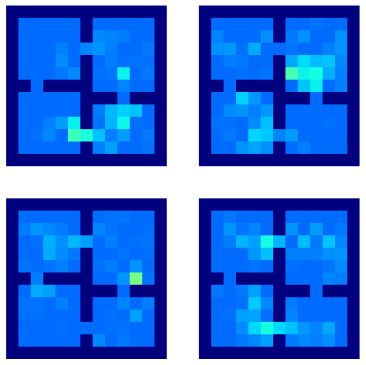
\includegraphics[width=4cm]{images/option-critic-4room.png}
    \caption{Termination probabilities for the option-critic
agent learning with 4 options (image from \cite{bacon_option-critic_2016}). \small \it Lighter colors encode higher termination probabilities.}
    \label{fig:opt-crit}
\end{wrapfigure}

An important contribution of this method is the option discovery method: the agent's behaviour is learned end-to-end through the optimization problem. Using a Boltzmann policies to parametrize the options, the authors solve the four-rooms navigation problem presented earlier. The termination probabilities for the each option are displayed in figure \ref{fig:opt-crit}. The highest spots are clustered near the hallways: it turns out that the agent learned a meaningful options structure that corresponds to the underlying abstract state space.

As a gradient-based method, the option-critic architecture lends itself to deep learning integration. In \cite{bacon_option-critic_2016} the authors test their method in the Arcade Learning Environment. The options and the overall policy parameters were learned through a convolutional neural network, and converged toward better performances than a classical DQN.

% Interestingly, the option-critic did not converge faster as other methods, since the first learning phase had to determine both the options structure and the policy over options. However, when abruptly changing the goal of the RL problem (in the four-rooms problem, moving the terminal state), it converged much faster toward the optimal policy, since it only had to learn a new $\pi_\Omega$.

As mentioned in \cite{alexander_strategic_2016} and \cite{vezhnevets_feudal_2017}, this architecture was only tested on relatively easy examples, thus the performance on harder problems like Atari games with rare rewards remains an open question.

\subsubsection{Feudal Networks}

In 2017, Vezhnevets \etal~\cite{vezhnevets_feudal_2017}, the authors adapt the feudal RL paradigm originally introduced in \cite{dayan_feudal_1993} into a new deep learning architecture, the FeUdal Network (FuN). The main idea they take stock on is that of a Manager giving goals and rewards to a Worker. In their paper, only one abstraction level is considered, but the approach can theoretically scale up to higher abstraction layers.

At each time step, the Manager and the Worker both receive a preprocessed state $z_t$. The manager encodes this state into a internal latent state $s_t(z_t)$. This internal state is fed into a recurrent neural network (RNN) which outputs a goal $g_t(s_t, s_{t-1}, ...)$, which is a high-dimensional vector. The moving average $w_t(g_t, ..., g_{t-k})$ of the last goals is transmitted with a linear transform to the Worker. On the Worker's side, the observation $z_t$ is fed into another RNN and produces a matrix $U_t(z_t, z_{t-1}, ...)$. The actions probabilities are then defined by $a_t = \mathrm{SoftMax}(U_t \times w_t)$. The pipeline is summed up in figure \ref{fig:fun}.

\begin{wrapfigure}{r}{7cm}
    \centering
    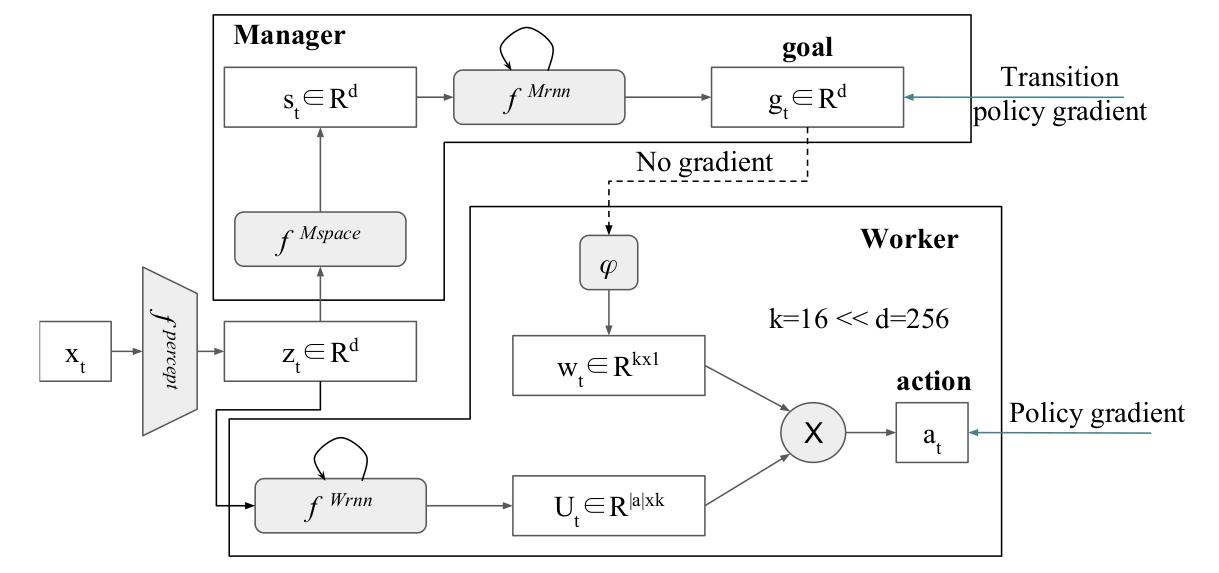
\includegraphics[width=7cm]{images/fun.png}
    \caption{The schema of a feudal network, reproduced from \cite{vezhnevets_feudal_2017}}
    \label{fig:fun}
\end{wrapfigure}

In the FuN, the Manager uses an internal state to generate a high-dimensional goal, which is given to the Worker, which has to try to this goal. Like in the original FRL setting, the reward $r_t$ is collected by the Manager. The Worker gets a pseudo-reward $r^W_t = r_t + \alpha r^M_t$ where $r^M_t = \frac 1T \sum_{i=0}^T d_\mathrm{cos}(s_t-s_{t-i}, g_{t-i})$, where $T$ is a time horizon and $d_\mathrm{cos}$ the cosine similarity. This means that the Manager considers that the Worker moves toward the goal iff its latent state evolves in the direction of the goal.

The Manager and Worker's parameters (for the input $z_t$ preprocessing, the Manager latent space $s_t$ embedding, the goal $g_t$ linear embedding and the RNNs) are learned through two distinct gradient steps (derived from variants of the classical policy gradient). This scheme hardcodes the distinction between the Manager and the Worker, thus preventing the optimization from considering the architecture as a monolithic model.

FuNs beats the performance achieved in the option-critic paper \cite{bacon_option-critic_2016} on similar experiments. They successfully discover advantageous subgoals and the related policies, and learn very fast compared with other recurrent approaches.

\subsection{}

\small
\bibliographystyle{unsrt}
\bibliography{HRL}

\end{document}